\documentclass[a4paper]{article}

\usepackage{amsmath}
\usepackage{tikz}
\usepackage[hidelinks]{hyperref}
\usepackage{xcolor}
\usepackage{colortbl}
\usepackage[a4paper, total={160mm, 240mm}]{geometry}
\usetikzlibrary{automata, positioning, arrows.meta, arrows}
\usepackage{graphicx}
\usepackage{float}
\usepackage{subcaption}  % Required for subfigures
\usepackage{caption}
\usepackage{booktabs}

\title{Written assignment (INL2): Problem solving with unsupervised learning}
\author{Mika Pärssinen and Marcus Hammarström}
\date{\today}

\begin{document}

\maketitle

\section{Problem formulation}

To get the most use of a football player, it is best to put them in a position where their specific set of skills shine. In our assignment we will try to predict what preferred position a football players has, based on their attributes. We will limit the classification problem to just outfield players, to classify a goalkeeper would be trivial. To achieve this we will use the given dataset, FIFA 18 Players database. The dataset has preferred positions labeled as a non-empty set of possible positions. Our problem will try and guess one of these positions.
\section{Sampling data}

\begin{itemize}
    \item Remove ``customer ID'' column from the dataset since it is not just an identifier for that unique feature vector.
    \item Remove ``tenure'' column from the dataset since we deem it might create noise in our data because the data is collected during a limited time.
    \item Remove the rows with missing values from the dataset.
\end{itemize}
\section{Normalization and outlier removal}

As part of the assignment, each pixel value has to be scaled down to the range $[0, 1]$. This is done by dividing each pixel value by $255.0$. This is done to feed our models with values that are they expect, the neurons in the networks except values in the range $[0, 1]$. The original pixel values are also in discrete integer values and the neural networks are work with continuous values.
\par
In terms of outliers, all appropiate preprocessing has been done and each image is considered to be equally important for classification. For this reason, no image is considered an outlier and no images are removed from the dataset.
\section{Hyperparameter selection}

\subsection{Hierarchical clustering}

The chosen hyperparameters for the Hierarchical clustering model are as follows:

\begin{itemize}
    \item \textbf{Method = Ward:} Because our data is numerical, and we want compact clusters the method choice is straight forward. Ward's method minimizes the total within cluster variance which results in compact and homogeneous clusters.
    
    \item \textbf{Metric = Euclidean:} Ward's method requires the use of the distance function Euclidean, when comparing alternative methods (average, complete, etc) with other distance functions we do not observe similarly effective cluster separations. Therefore strengthening our choice of Ward's method and Euclidean distance.
    \item \textbf{Number of clusters = 5:} The number of clusters is chosen by creating and analyzing a dendogram, where the number of clusters is determined by drawing a horizontal line at the top of the dendogram. The horizontal line is placed so the distances between horizontal lines above are big, indicating that each cluster is far apart from eachother. We also consider the silhouette score of different amonunt of clusters. We choose 5 clusters, but discussions with domain experts about our clustering results could lead to a different number of clusters. Silhouette score bar plot and dendogram can be seen in \autoref{fig:silhouette_agglomerative} and \autoref{fig:dendogram} below:
\end{itemize}

\begin{figure}[H]
    \hspace*{\fill}
    \centering
    \begin{subfigure}[b]{0.45\textwidth}
        \centering
        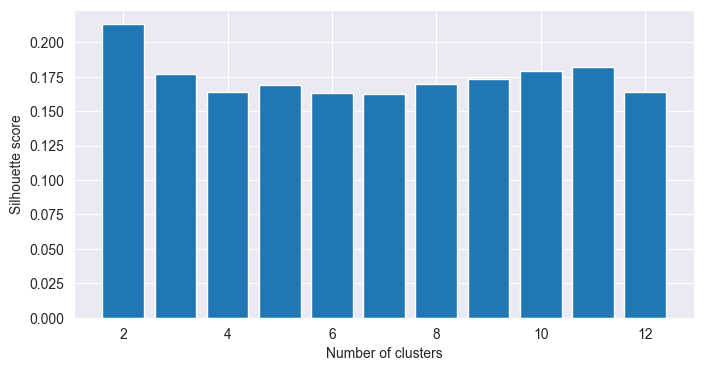
\includegraphics[width=1.0\textwidth]{src/figs/silhouette_agglomerative.png} 
        \caption{Silhouette scores for agglomerative clustering}\label{fig:silhouette_agglomerative}
    \end{subfigure}
    \hfill
    \begin{subfigure}[b]{0.45\textwidth}
        \centering
        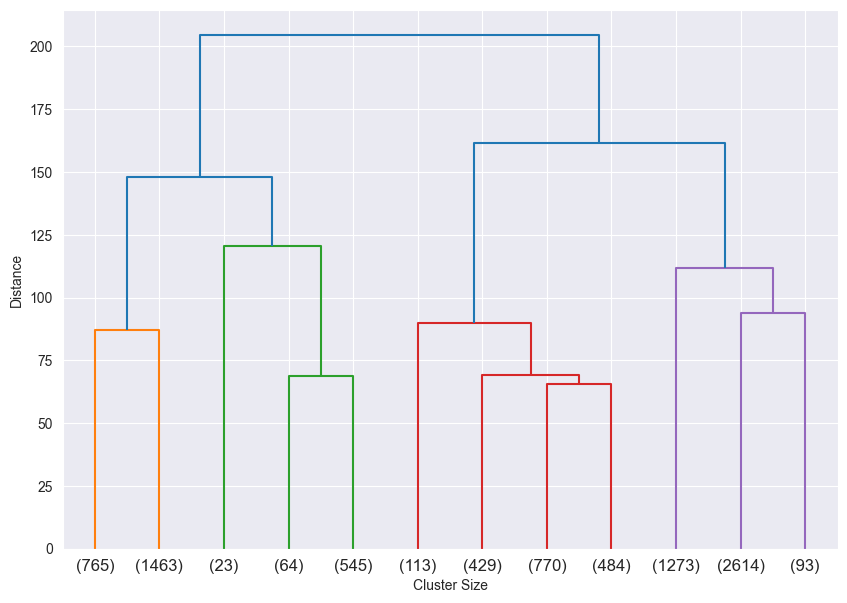
\includegraphics[width=1.0\textwidth]{src/figs/dendogram.png} 
        \caption{Dendogram}\label{fig:dendogram}
    \end{subfigure}\label{fig:silhouette_dendogram}
    \caption{Hierarchical clustering hyperparameter selection}\label{fig:hyperparameters_hierarchical}
    \hspace*{\fill}
\end{figure}



\subsection{DBSCAN}

The chosen hyperparameters for the DBSCAN model are as follows:

\begin{itemize}
    \item \textbf{Min samples = 17:} A rule of thumb for choosing min\_samples is to set it to be the number of features in the dataset plus one. In our case, we have $16$ features, so we set min\_samples to $17$.
    \item \textbf{Epsilon = 0.3:} The epsilon value is chosen by first calculating the distance of each point to it's $17$-th nearest neighbor. Choosing $17$-th nearest in our case because that is our min\_samples. We then plot a histogram to find a knee to define an appropriate epsilon value. The histogram can be seen in \autoref{fig:epsilon_histogram} below. The knee seems to be found at somewhere between $0.25$ and $0.35$. To chose a good value between these two, we also look at the silhouette score for the different epsilon values, found in \autoref{fig:silhouette_epsilon}. We choose $0.3$ as our epsilon value.
\end{itemize}

\begin{figure}[H]
    \hspace*{\fill}
    \centering
    \begin{subfigure}[b]{0.45\textwidth}
        \centering
        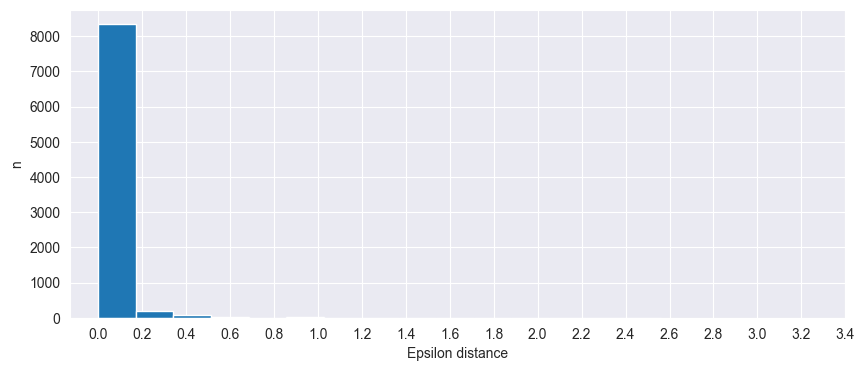
\includegraphics[width=1.0\textwidth]{src/figs/epsilon_histogram.png} 
        \caption{Epsilon value histogram}\label{fig:epsilon_histogram}
    \end{subfigure}
    \hfill
    \begin{subfigure}[b]{0.45\textwidth}
        \centering
        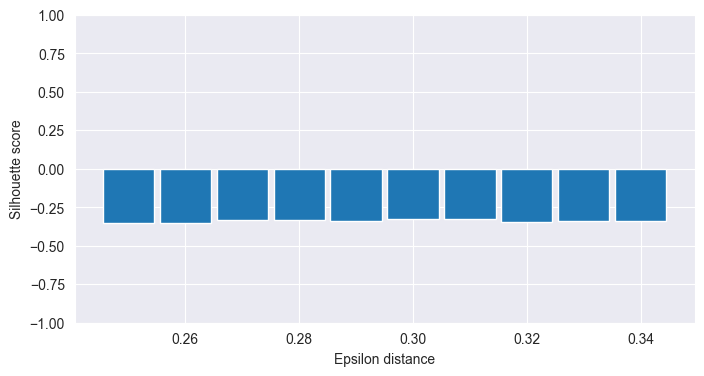
\includegraphics[width=1.0\textwidth]{src/figs/silhouette_epsilon.png} 
        \caption{Silhouette scores for different epsilon values}\label{fig:silhouette_epsilon}
    \end{subfigure}
    \caption{Epsilon hyperparameter selection}\label{fig:hyperparameters_dbscan}
    \hspace*{\fill}
\end{figure}

\section{Model selection}

\section{Metrics used for evaulation}

The evaluation metrics used for classification is quite straight forward, we will measure accuracy in terms of how many predicted labels are correct over the total amount of test labels. What we do do different from a standard labeling procedure is what we consider is labeling test data correctly. The regular labeling process consider a prediction correct if the predicted label is an exact match with the test label. But what we consider an accurate prediction is if the label is a subset of the set of possible positions for the player.
\vspace{-0.2cm}
\section{Result}
\vspace{-0.1cm}
\subsection{Hierarchical Clustering}

\subsubsection{Evaluation}

\begin{figure}[H]
    \centering
    \begin{tabular}{|l|c|}
        \hline
        \rowcolor{gray!50}
        & Value \\ \hline
        \textbf{Silhouette Score} & $0.169$ \\ \hline
        \textbf{Dunn Index} & $0.009$ \\ \hline
    \end{tabular}
    \vspace{-0.1cm}
    \caption{Evaluation metrics for Hierarchical Clustering}\label{fig:Hierarchical_evaluation}
    \vspace{-0.2cm}
\end{figure}
%\vspace{-0.1cm}
\subsubsection{Visualization of the clusters:}
\begin{figure}[H]
    \centering
    \begin{subfigure}[b]{0.45\textwidth}
        \centering
        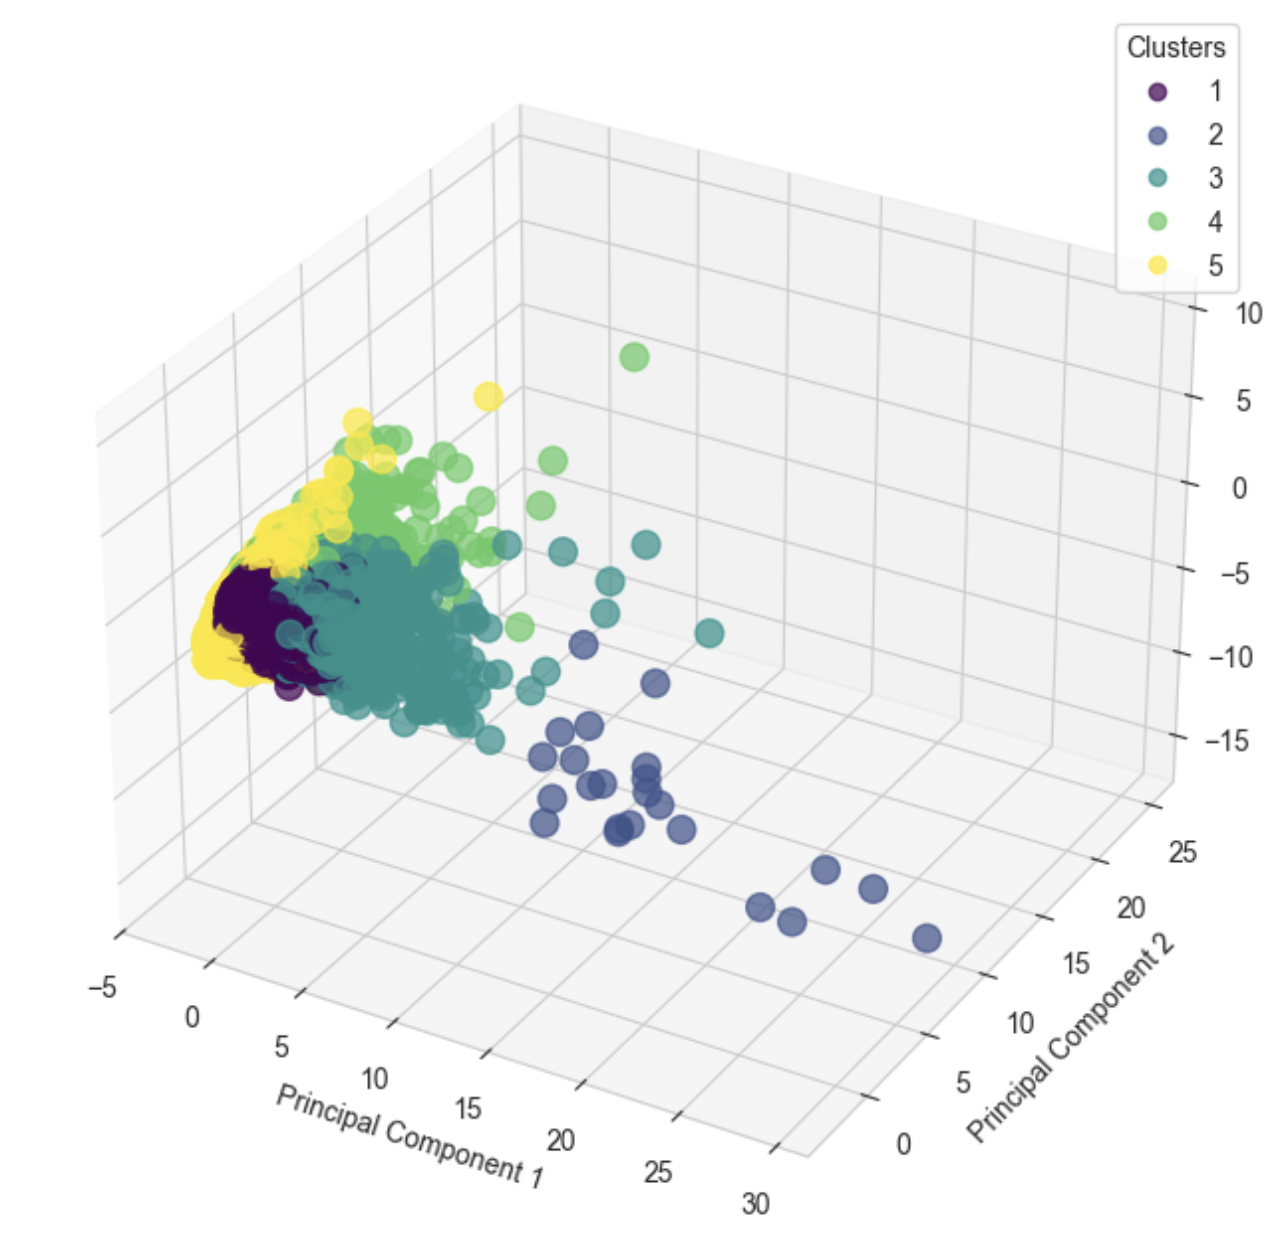
\includegraphics[width=\textwidth]{src/figs/3d_PCA_HC.png}
        \caption{3D PCA}
        \label{fig:3D_pca}
    \end{subfigure}
    \hfill
    \begin{subfigure}[b]{0.45\textwidth}
        \centering
        \raisebox{0.3cm}{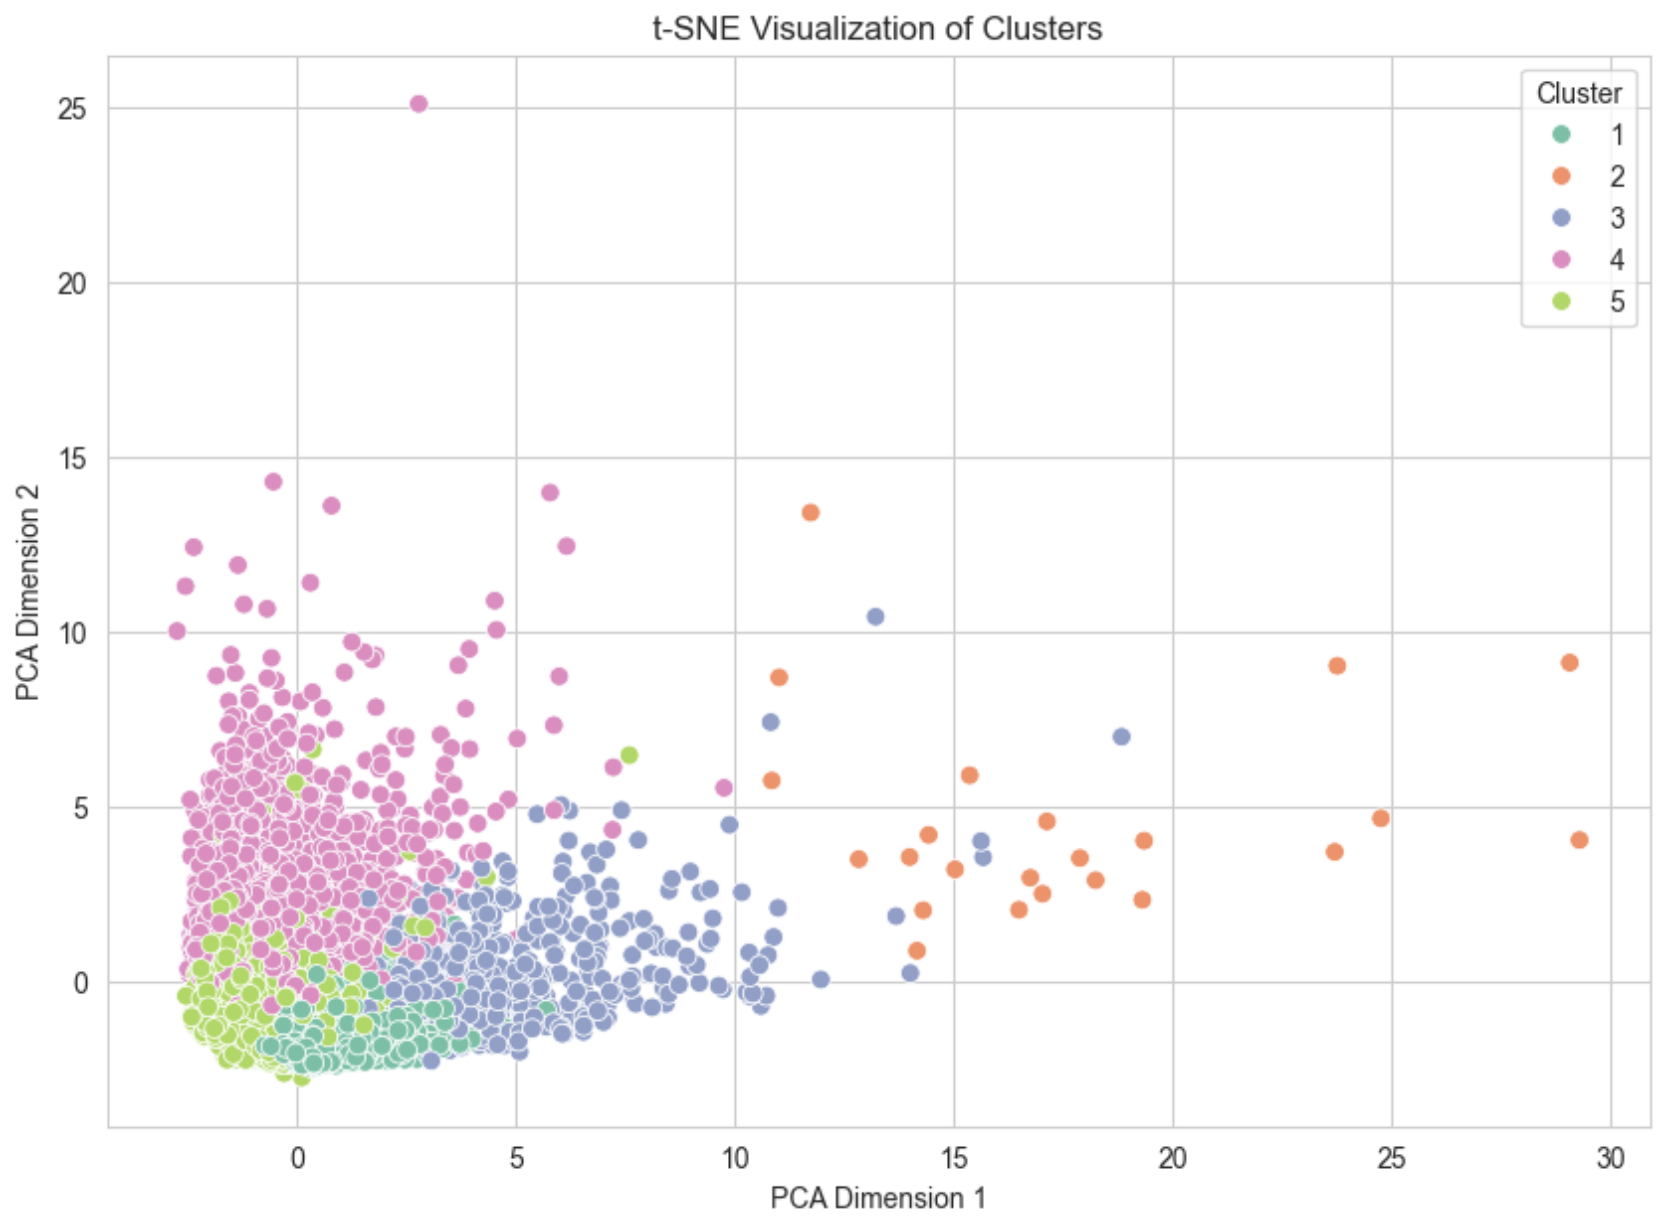
\includegraphics[width=\textwidth]{src/figs/2d_PCA_HC.png}} % Adjusts the image height
        \caption{2D PCA}
        \label{fig:PCA_2d}
    \end{subfigure}
    \caption{Clustering visualizations: 3D (left) and 2D (right).}
    \label{fig:comparison1}
\end{figure}

\begin{figure}[H]
    \centering
    \begin{subfigure}[b]{0.45\textwidth}
        \centering
        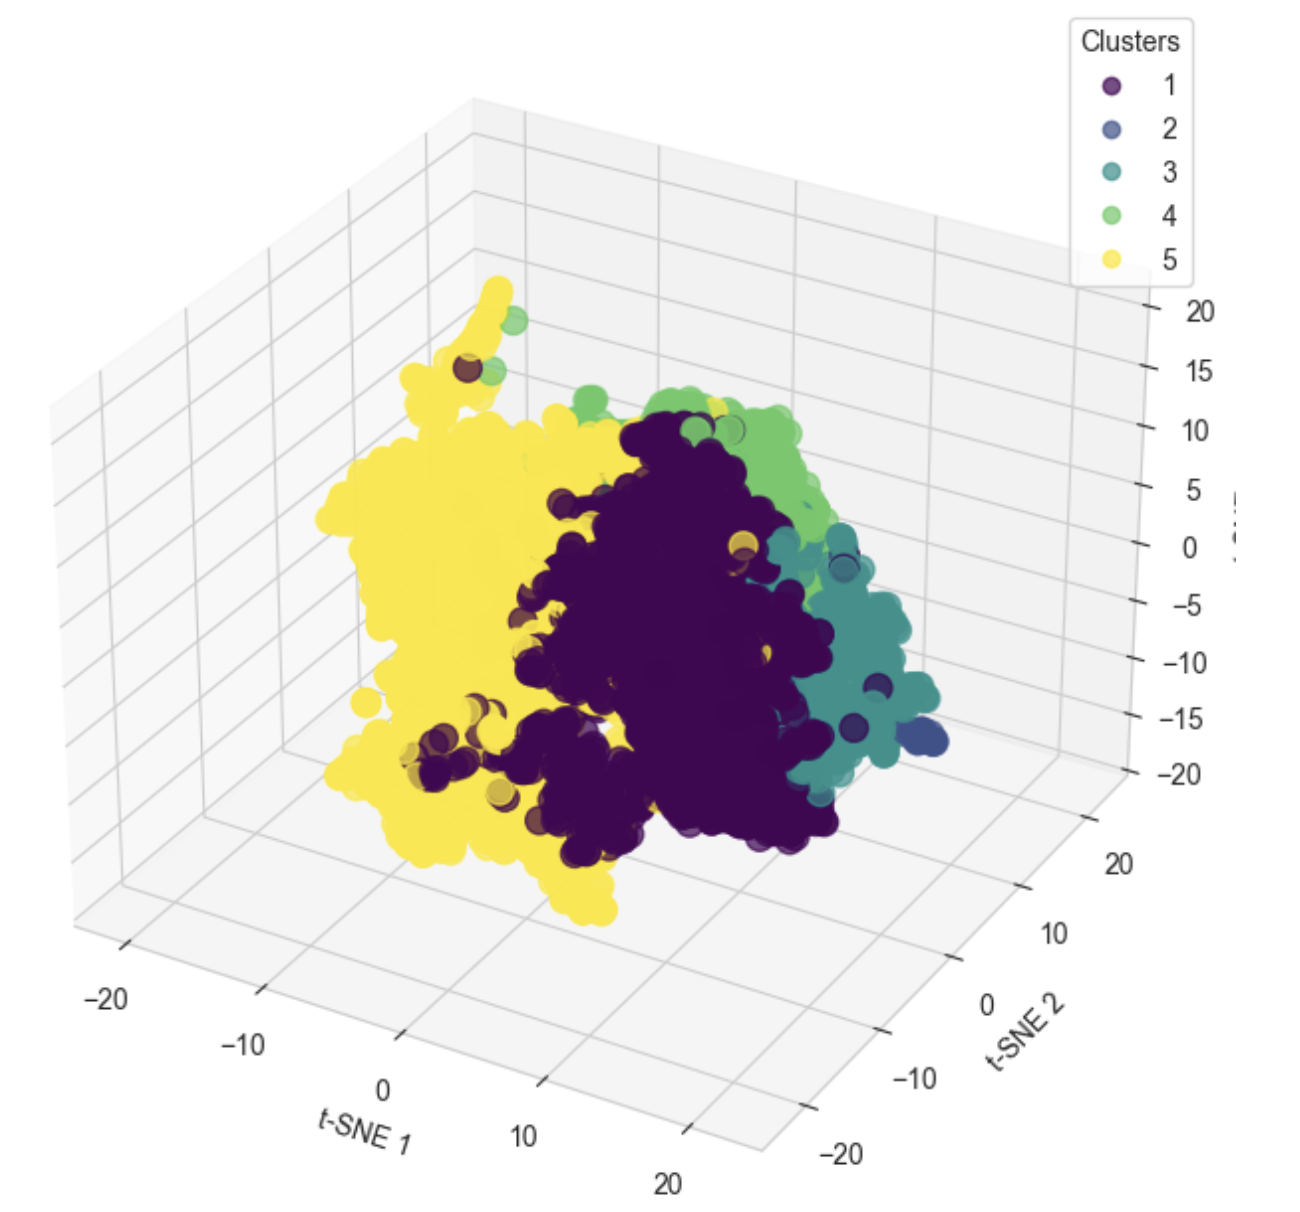
\includegraphics[width=\textwidth]{src/figs/3d_t-SNE.png}
        \caption{3D t-SNE}
        \label{fig:3D_tsne}
    \end{subfigure}
    \hfill
    \begin{subfigure}[b]{0.45\textwidth}
        \centering
        \raisebox{0.3cm}{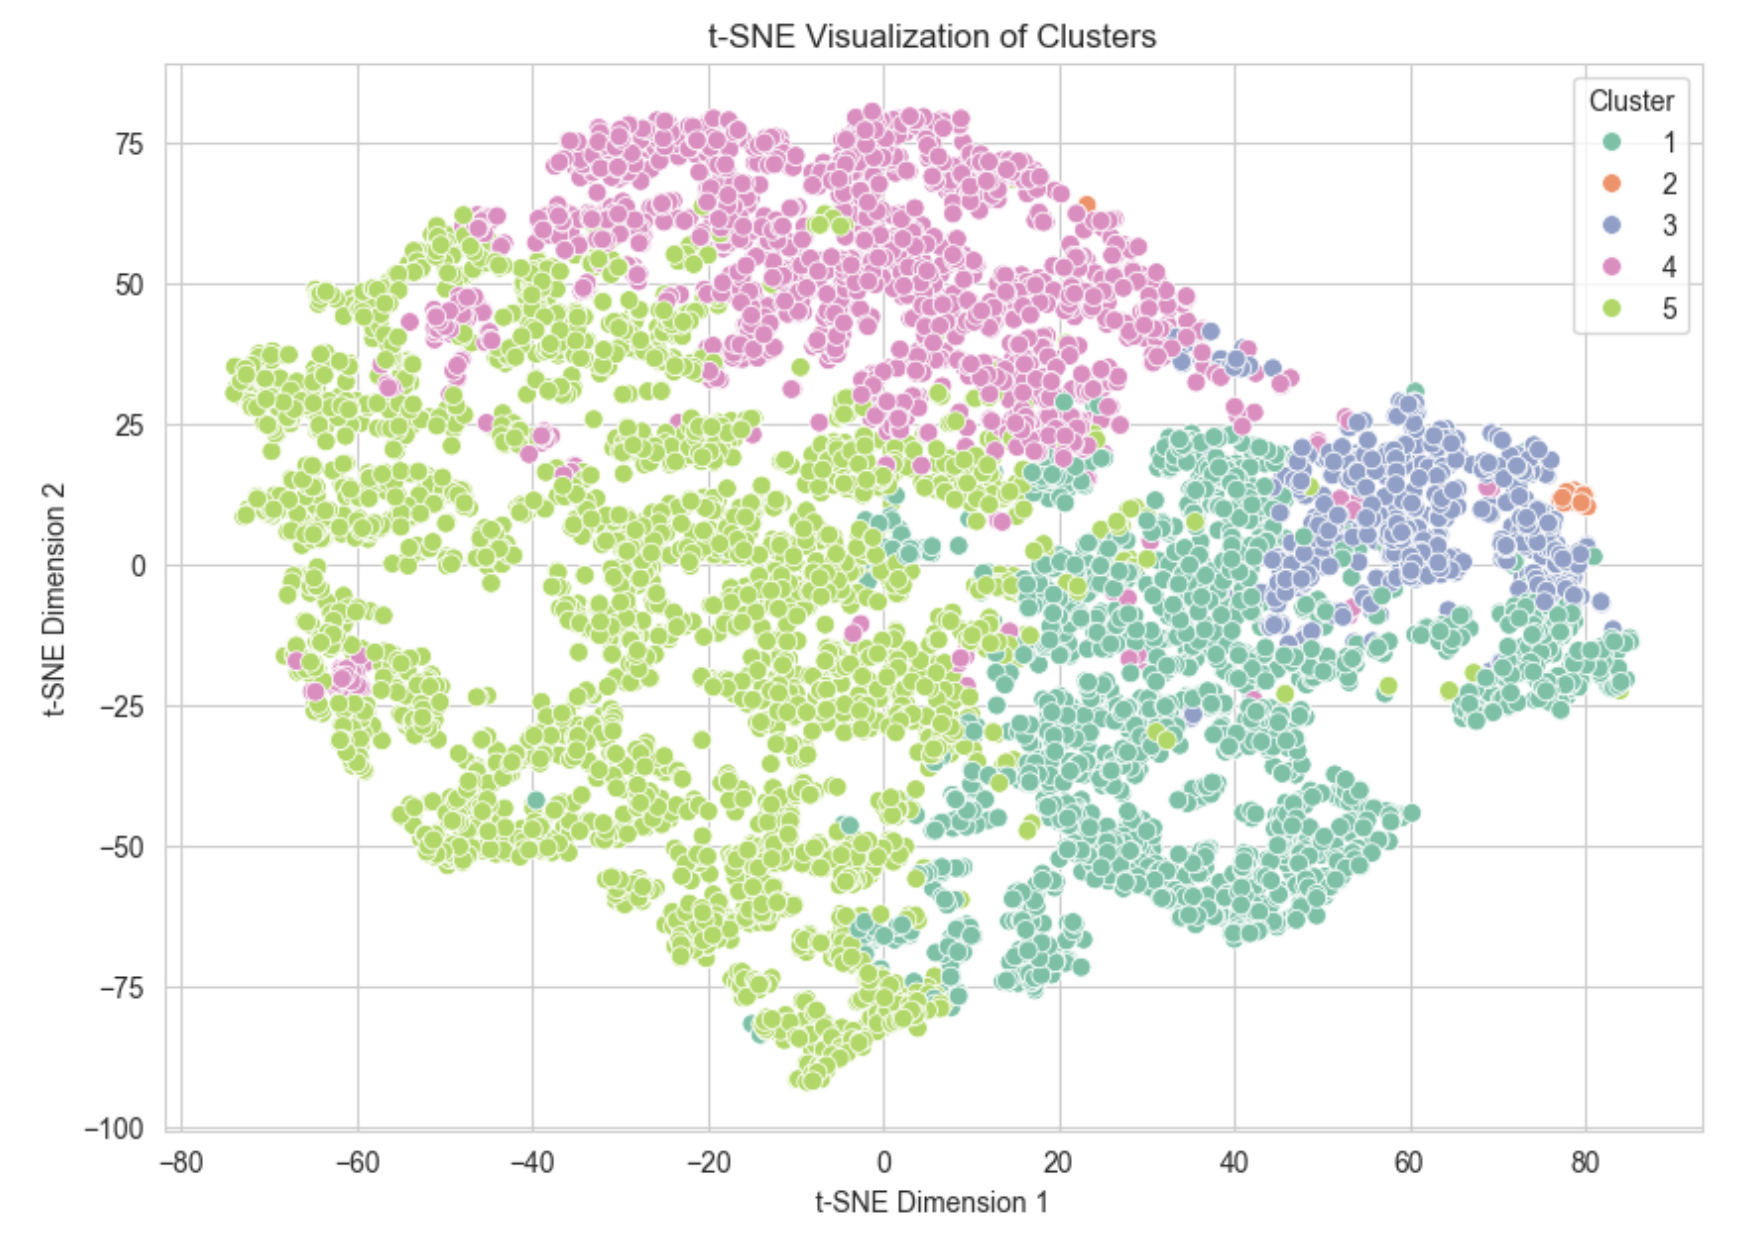
\includegraphics[width=\textwidth]{src/figs/2d_t-SNE.png}} % Adjusts the image height
        \caption{2D t-SNE}
        \label{fig:2D_tsne}
    \end{subfigure}
    \caption{Clustering visualizations: 3D (left) and 2D (right).}
    \label{fig:comparison2}
\end{figure}

\subsubsection{Cluster Descriptions}
Clarification on what the clusters contain and represent.
Values are represented by the mean of each cluster, except for the cluster size, which is calculated as the sum of all data points in the cluster.  

\vspace{0.3cm}
\par

\begin{center}


\noindent
\begin{minipage}[t]{0.48\textwidth}
\centering
\textbf{Cluster 1: Medium Activity, Low Spenders with Higher Full Payment Rate}
\vspace{0.2cm}
\resizebox{\textwidth}{!}{
\begin{tabular}{|l|c|c|}
\hline
\rowcolor{gray!50}
\textbf{Feature} & \textbf{Values} & \textbf{Interpretation} \\ \hline
Balance & 587.98 & Low \\ \hline
Purchases & 1203.26 & Low \\ \hline
One-Off Purchases & 542.97 & Moderate \\ \hline
Installments Purchases & 660.38 & Moderate \\ \hline
Cash Advance & 69.96 & Low \\ \hline
Credit Limit & 4157.06 & Moderate \\ \hline
Payments & 1269.62 & Moderate \\ \hline
Full Payment Percentage & 0.35 & Moderate \\ \hline
Cluster size & 2228.00 & Moderate \\ \hline
\end{tabular}}
\captionof{table}{Cluster 1 description.}
\end{minipage}
\hfill
\begin{minipage}[t]{0.48\textwidth}
\centering
\textbf{Cluster 2: High Spenders with Large Balances and High Full Payment Rate}
\vspace{0.2cm}
\resizebox{\textwidth}{!}{
\begin{tabular}{|l|c|c|}
\hline
\rowcolor{gray!50}
\textbf{Feature} & \textbf{Values} & \textbf{Interpretation} \\ \hline
Balance & 4812.38 & Very High \\ \hline
Purchases & 27505.34 & Very High \\ \hline
One-Off Purchases & 22417.45 & Very High \\ \hline
Installments Purchases & 5087.89 & Very High \\ \hline
Cash Advance & 1617.79 & High \\ \hline
Credit Limit & 16000.00 & Very High \\ \hline
Payments & 28138.98 & Very High \\ \hline
Full Payment Percentage & 0.53 & High \\ \hline
Cluster size & 23.00 & Very Low \\ \hline
\end{tabular}}
\captionof{table}{Cluster 2 description.}
\end{minipage}

\vspace{0.7cm}

\noindent
\begin{minipage}[t]{0.48\textwidth}
\centering
\textbf{Cluster 3: Moderate Credit Usage with Low Full Payment Rate}
\vspace{0.2cm}
\resizebox{\textwidth}{!}{
\begin{tabular}{|l|c|c|}
\hline
\rowcolor{gray!50}
\textbf{Feature} & \textbf{Values} & \textbf{Interpretation} \\ \hline
Balance & 3093.29 & High \\ \hline
Purchases & 5059.38 & Moderate \\ \hline
One-Off Purchases & 3176.73 & Moderate \\ \hline
Installments Purchases & 1883.64 & Moderate \\ \hline
Cash Advance & 427.99 & Moderate \\ \hline
Credit Limit & 8084.07 & High \\ \hline
Payments & 4411.09 & Moderate \\ \hline
Full Payment Percentage & 0.18 & Low \\ \hline
Cluster size & 609.00 & Low \\ \hline
\end{tabular}}
\captionof{table}{Cluster 3 description.}
\end{minipage}
\hfill
\begin{minipage}[t]{0.48\textwidth}
\centering
\textbf{Cluster 4: Customers with Low Purchases, High Cash Advances, and Low Full Payment}
\vspace{0.2cm}
\resizebox{\textwidth}{!}{
\begin{tabular}{|l|c|c|}
\hline
\rowcolor{gray!50}
\textbf{Feature} & \textbf{Values} & \textbf{Interpretation} \\ \hline
Balance & 3753.04 & High \\ \hline
Purchases & 536.14 & Low \\ \hline
One-Off Purchases & 311.82 & Low \\ \hline
Installments Purchases & 224.39 & Low \\ \hline
Cash Advance & 3412.73 & Very High \\ \hline
Credit Limit & 6304.57 & High \\ \hline
Payments & 2908.71 & Low \\ \hline
Full Payment Percentage & 0.04 & Low \\ \hline
Cluster size & 1796.00 & Moderate \\ \hline
\end{tabular}}
\captionof{table}{Cluster 4 description.}
\end{minipage}

\vspace{0.7cm}


\noindent
\begin{minipage}[t]{0.48\textwidth}
\centering
\textbf{Cluster 5: Low Usage of Credit with Minimal Purchases or Payments}
\vspace{0.2cm}
\resizebox{\textwidth}{!}{
\begin{tabular}{|l|c|c|}
\hline
\rowcolor{gray!50}
\textbf{Feature} & \textbf{Values} & \textbf{Interpretation} \\ \hline
Balance & 950.55 & Low \\ \hline
Purchases & 376.41 & Low \\ \hline
One-Off Purchases & 252.25 & Low \\ \hline
Installments Purchases & 124.60 & Low \\ \hline
Cash Advance & 503.19 & Low \\ \hline
Credit Limit & 3310.72 & Low \\ \hline
Payments & 1011.16 & Low \\ \hline
Full Payment Percentage & 0.10 & Low \\ \hline
Cluster size & 3980.00 & High \\ \hline
\end{tabular}}
\captionof{table}{Cluster 5 description.}
\end{minipage}

\end{center}


\subsection{DBSCAN}

\subsubsection{Evaluation}

\begin{figure}[H]
    \centering
    \begin{tabular}{|l|c|}
        \hline
        \rowcolor{gray!50}
        & Value \\ \hline
        \textbf{Silhouette Score} & $-0.328$ \\ \hline
        \textbf{Dunn Index} & $0.001$ \\ \hline
    \end{tabular}
    \caption{Evaluation metrics for DBSCAN}\label{fig:DBSCAN_evaluation}
\end{figure}

\subsubsection{Visualization of the clusters:}

The clusters we get from DBSCAN are visualized in 3D using PCA and t-SNE. First we visualize the clusters including the $-1$ cluster, which represents the outliers. Then we visualize the clusters without the $-1$ cluster, to get a better view of the clusters that DBSCAN finds.

\begin{figure}[H]
    \hspace*{\fill}
    \centering
    \begin{subfigure}[b]{0.45\textwidth}
        \centering
        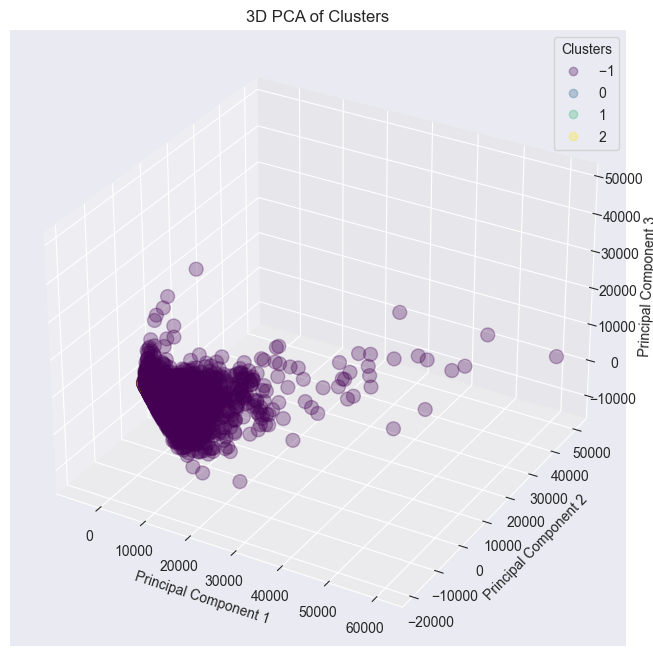
\includegraphics[width=1.0\textwidth]{src/figs/3d_PCA_DBSCAN_with.png} 
        \caption{3D PCA with $-1$ cluster}\label{fig:DBSCAN_PCA_with}
    \end{subfigure}
    \hfill
    \begin{subfigure}[b]{0.45\textwidth}
        \centering
        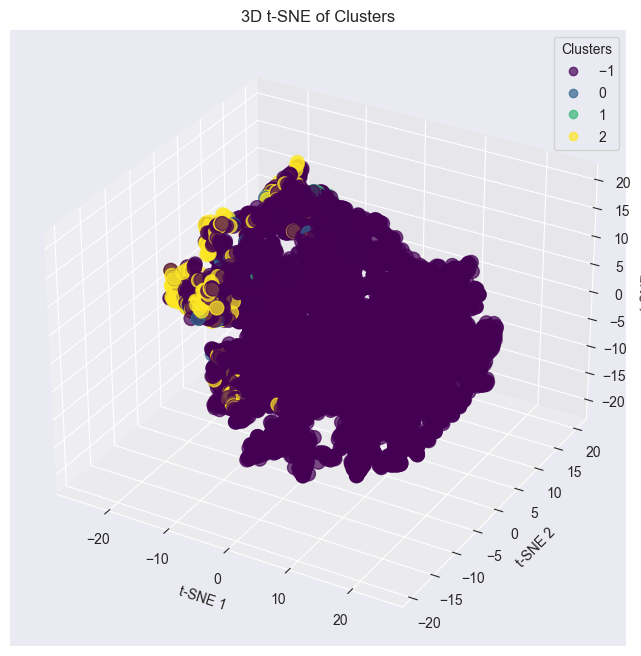
\includegraphics[width=1.0\textwidth]{src/figs/3d_t-SNE_DBSCAN_with.png} 
        \caption{3D t-SNE with $-1$ cluster}\label{fig:DBSCAN_tsne_with}
    \end{subfigure}
    \caption{Visualization of DBSCAN clusters with $-1$ cluster data included}\label{fig:with_outliers}
    \hspace*{\fill}
\end{figure}

\begin{figure}[H]
    \hspace*{\fill}
    \centering
    \begin{subfigure}[b]{0.45\textwidth}
        \centering
        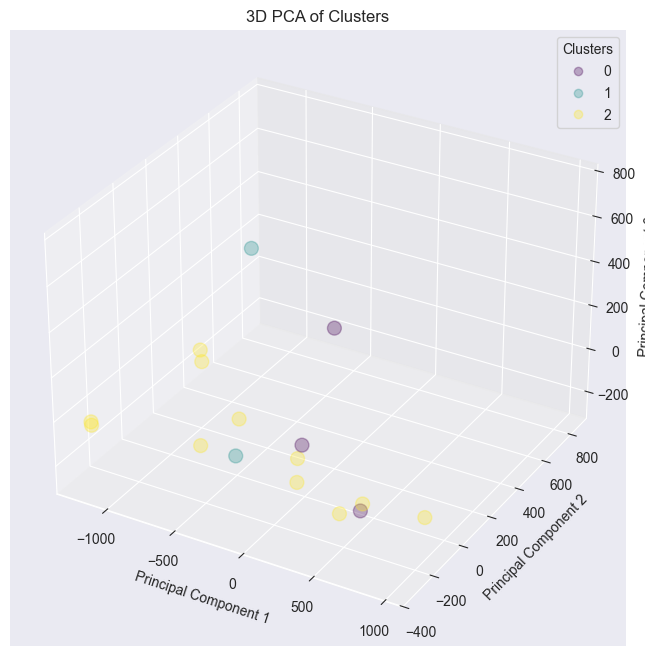
\includegraphics[width=1.0\textwidth]{src/figs/3d_PCA_DBSCAN_without.png} 
        \caption{3D PCA without $-1$ cluster}\label{fig:DBSCAN_PCA_without}
    \end{subfigure}
    \hfill
    \begin{subfigure}[b]{0.45\textwidth}
        \centering
        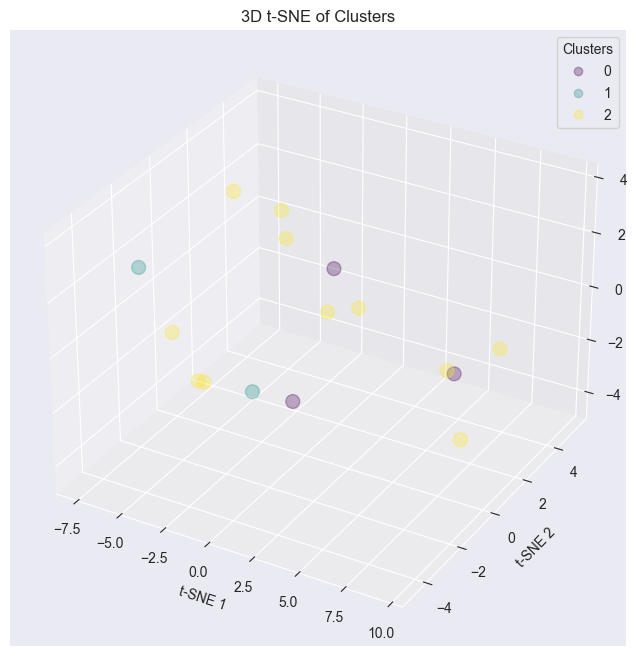
\includegraphics[width=1.0\textwidth]{src/figs/3d_t-SNE_DBSCAN_without.png} 
        \caption{3D t-SNE without $-1$ cluster}\label{fig:DBSCAN_tsne_without}
    \end{subfigure}
    \caption{Visualization of DBSCAN clusters with $-1$ cluster data excluded}\label{fig:without_outliers}
    \hspace*{\fill}
\end{figure}
\section{Discussion}

\subsection{Ethical consideration}

Our implementation of a machine learning model to classify bottles in a factory brings a few important ethical considerations. 
While the technology offers great improvements in quality control and efficiency, it also presents challenges that need to be discussed and thought about.

First of is data security and privacy. 
The system processes large amounts of production data that could be valuable to competitors. 
Factories that uses our implementation is therefore recommended to implement a robust cybersecurity system to protect against industrial espionage and unauthorized access. 
This includes secure data storage, encrypted communications, and strict access controls for system modifications.

Additionally, our implementation leads to workforce changes. While some traditional quality control positions may be displaced, new roles emerge in system maintenance, monitoring, and data analysis. 
This transformation requires human resources, they should present retraining programs and use clear communication with affected employees.
To ensure employees gets the right and fair treatment.

Finally, accountability and responsibility of our implementation present another critical consideration. 
If defective products reach customers, clear frameworks must be establish whether responsibility lies with the system developers, factory management, or quality control staff. 
This requires transparent documentation of the system's decision-making process and regular reviews of its performance.

In conclusion, ethical implications of implementing this technology extend beyond the factory product line.
While automation can improve product quality and reduce waste, organizations must balance these benefits against their social responsibilities. 
This includes maintaining employment opportunities while adapting to technological advancement, ensuring transparent communication with stakeholders, and maintaining human oversight in critical decision-making processes.

\subsection{Limitations}

• Inte riktig data
• Fake noise, riktigt noise skulle vara damm och smuts på linsen tex.
\section{Conclusion}

Our paper demonstrates the effectiveness of an autoencoder-based anomaly detection system combined with a CNN for classifying bottle defects, while still using a small dataset.
The anomaly detection procedure accurately identifies anomalies with minimal errors, and the CNN successfully classifies the defects. 
However, consider the limitations such as reliance on synthetic data, overrepresentation of a certain class, and the introduction of synthetic noise may affect the performance in the real world.
While the model performs well in a controlled setting, its generalizability to actual factory conditions remains unknown.

Future improvements include testing alternative architectures, enhancing data augmentation techniques, and deploying the model in a real production environment to collect authentic defect data. 
Ethical considerations such as data security, workforce impact, and accountability must also be addressed when implementing such systems in industry. 
Overall, this paper highlights the potential of deep learning for automated defect detection, but further validation by applications in the real world is necessary to ensure reliability and robustness.

\end{document}